\begin{thm}{145}{\hosi ?}{}
 \begin{enumerate}
  \item 以下の画像は正五角形ABCDEと、その対角線の交点F, G, H, I, Jである。$\mr{AB}=1$のとき、FGの値を求めよ。
  \item (1)の結果から、$\sin 72^\circ$, $\cos 72^\circ$, $\sin 36^\circ$, $\cos 36^\circ$ を求めよ。
 \end{enumerate}
 \begin{center}
  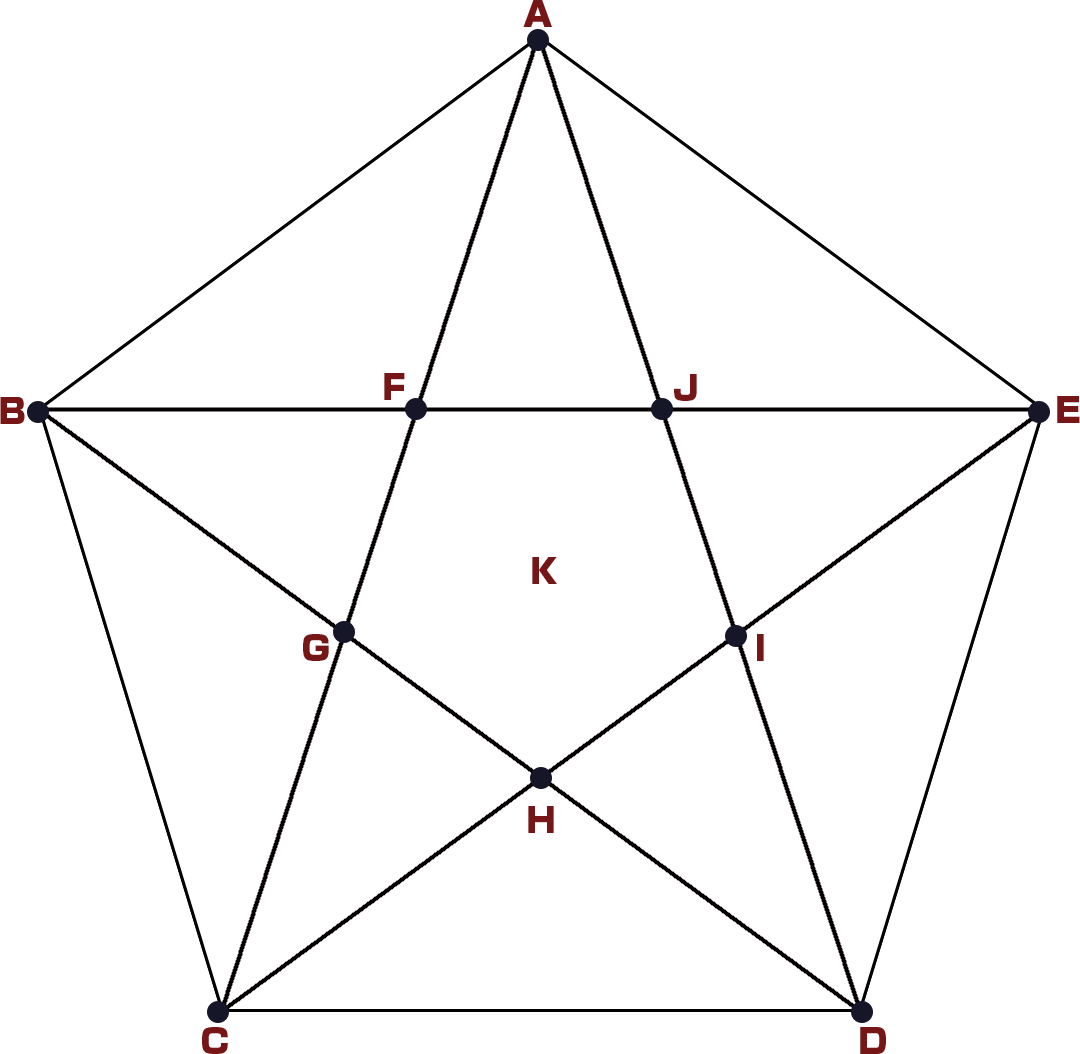
\includegraphics[bb=0 0 1080 1054,width=0.7\linewidth]{../problems/Q_145/Q_145.png}
 \end{center}
\end{thm}

\syoumon{1}
ここに解答を記述。

\syoumon{2}
ここに解答を記述。